\chapter{Мотор-колеса в составе автомобиля} \label{ch:ch1}

\section{Топологии электромобилей} \label{sec:ch1/sec1}

%Мы можем сделать \textbf{жирный текст} и \textit{курсив}.
Электромобили в настоящее время рассматриваются как наиболее перспективный вид транспортного средства. Причиной этому служит ряд его преимуществ: Отсутствие вредных выбросов во время движения, низкий шум, а также высокий крутящий момент на старте. Однако, на данный момент, электромобили сильно уступают транспортным средствам с двигателями внутреннего сгорания (ДВС) по максимальному запасу хода. В условиях ограниченного запаса емкости аккумуляторных батарей (АБ) на борту электромобиля возникает необходимость в разработке наиболее энергоэффективной, легкой и компактной тяговой установки, чтобы увеличить максимальный запас хода электромобиля на одном заряде. 
На данный момент можно выделить два основных способа достичь максимального значения удельной мощности (отношения сумм мощностей тяговых агрегатов к конечному весу автомобиля) и максимальной эффективности трансмиссии электромобиля. Первый способ (рисунок \ref{fig:nomr}) заключается в установке высокоскоростного электромотора (так как их вес и габариты существенно ниже, чем у моторов с более низкой скоростью и эквивалентной мощностью). Однако недостатком такого способа является наличие механических потерь в трансмиссии, что сильно снижает общую эффективность топологии.
Более простым и эффективным способом повышения удельной мощности транспортного средства является использование мотор-колес: высоко-моментных, низкоскоростных моторов, установленных внутри колес автомобиля (рисунок \ref{fig:mr}). Подробно данный тип электромоторов был рассмотрен в \cite{1Luque}[1]. Использование мотор-колес в трансмиссии электротранспорта позволит достичь улучшения динамических характеристик электротранспорта, а также избавиться от таких частей трансмиссии как карданный вал, дифференциал и т.д. Это позволит снизить конечный вес агрегата, а также повысить общий КПД системы \cite{2KingJetTseng,3Lovatt}.
\noindent К основным достоинствам использования мотор-колес можно отнести::
\begin{enumerate}
	\item Независимое управление моментом и скоростью каждого колеса.
	\item Оптимизация места (более компактное расположение).
	%\item Третий пункт.
\end{enumerate}
На данный момент автомобили с мотор-колесами разрабатываются многими производителями \cite{4Jain,5Espanet}, в том числе в условиях бездорожья \cite{6Zhitkova}.
\begin{figure}[ht]
	\centering
	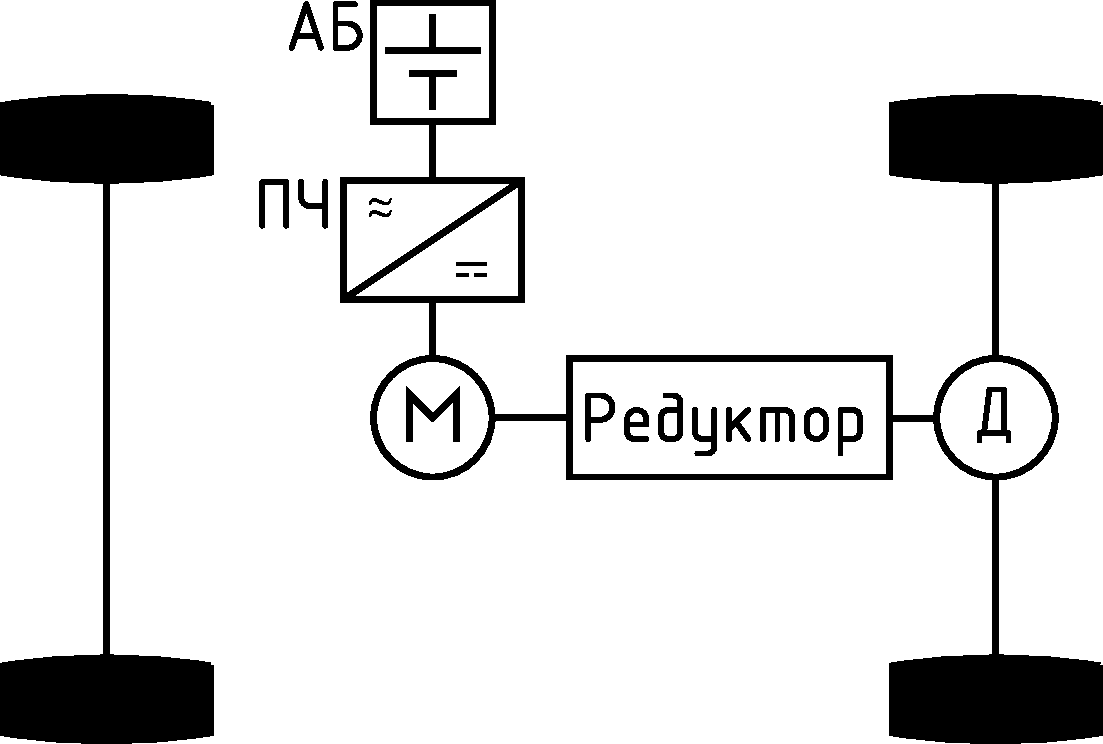
\includegraphics [scale=0.5] {nomr}
	\caption{Стандартная топология электротрансмиссии с одним мотором \cite{4Jain}}
	\label{fig:nomr}
\end{figure}


\begin{figure}[ht]
	\centering
	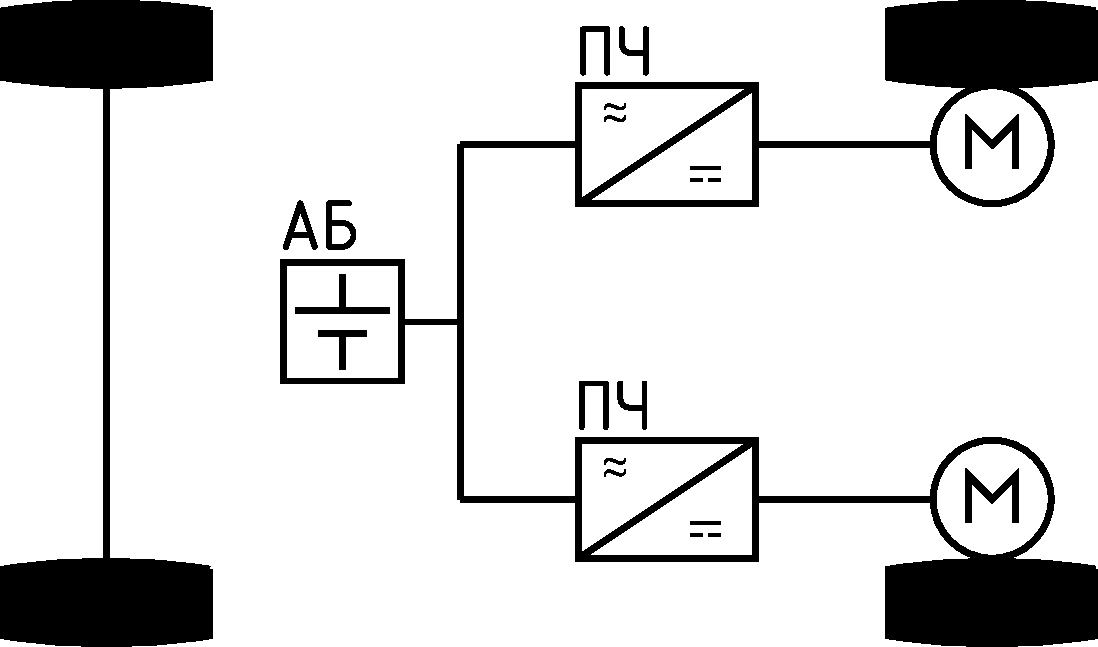
\includegraphics [scale=0.5] {mr}
	\caption{Топология электротрансмиссии с мотор-колесами \cite{4Jain}}
	\label{fig:mr}
\end{figure}

На рисунке \ref{fig:inwheel} изображено мотор-колесо, разработанное компанией Protean, а также его составные части. 
Однако, несмотря на вышеперечисленные достоинства, данный тип моторов имеет один недостаток – большая неподрессоренная масса, которая снижает комфорт от езды, а также уменьшает способность автомобиля удерживать заданное направление движения. Существуют различные способы решения данной проблемы \cite{7Tang}, однако их решение выходит за рамки поставленных в исследовании целей и задач.

\begin{figure}[ht]
	\centering
	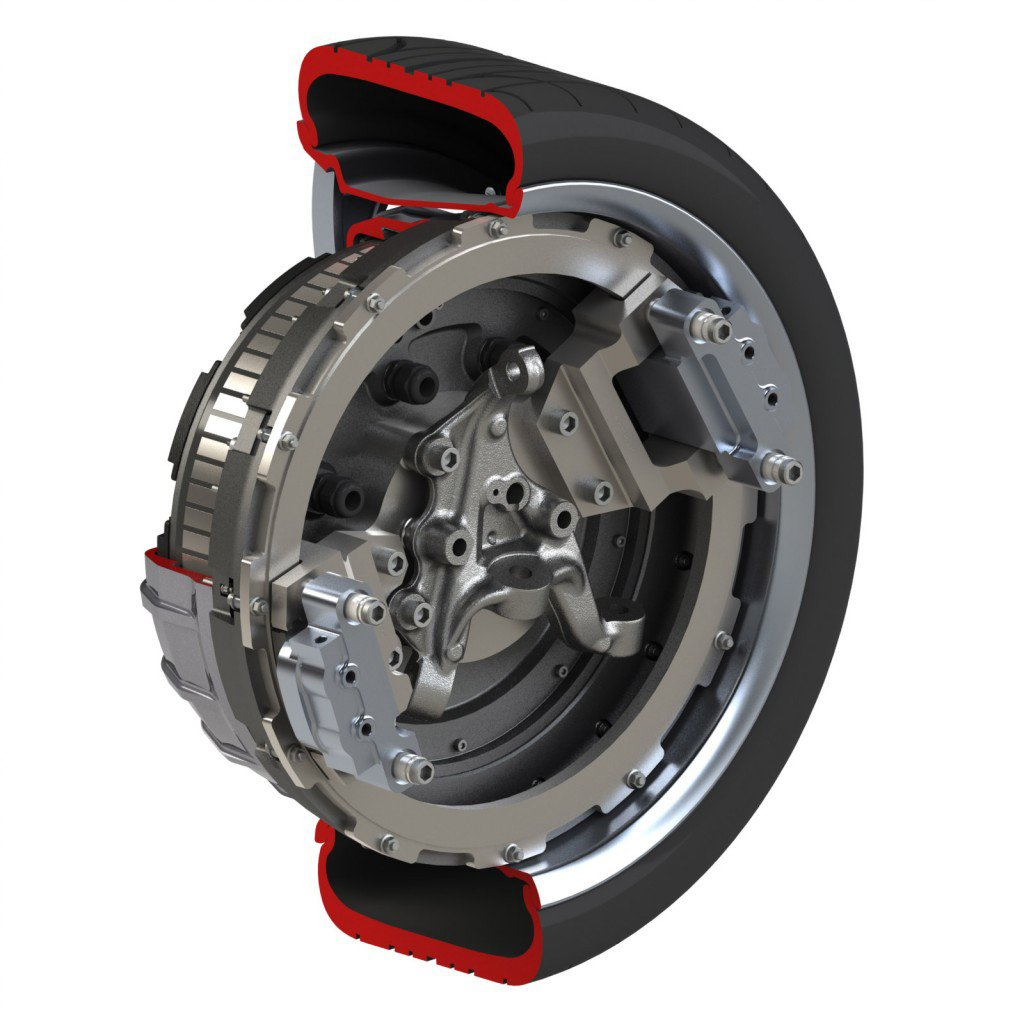
\includegraphics [scale=0.25] {inwheel}
	\caption{Мотор-колесо}
	\label{fig:inwheel}
\end{figure}

В составе мотор-колеса могут быть использованы различные типы электродвигателей. Данное исследование ориентировано на рассмотрение мотор-колес с синхронным электродвигателем с постоянными магнитами (СДПМ). Ниже будут рассмотрены основные достоинства и недостатки СПДМ в составе мотор-колес. 


\subsection{Синхронные двигатели с постоянными магнитами}
\noindent Основными требованиями для электромоторов в составе мотор-колес являются:
\begin{enumerate}
	\item Высокий крутящий момент на низких скоростях
	\item Широкий диапазон регулирования скорости
	\item Высокий коэффициент удельной мощности
\end{enumerate}

Низкий вес мотора – наиболее важный параметр, необходимый для достижения высоких динамических характеристик мотора вследствие уменьшения общей неподрессоренной массы электромобиля. Таким образом отношение КПД мотора к его весу – основной критерий выбора электромотора. \noindent Электродвигатели, соответствующие вышеобозначенным критериям, представлены следующими типами:
\begin{enumerate}
\item Асинхронный электродвигатель \cite{8Benoudjit,9FeiXu}
\item Синхронный двигатель с постоянными магнитами \cite{10Fan}
\item Бесщеточный двигатель постоянного тока (вентильный электродвигатель) \cite{11YeePienYang,12Miyamasu}
\item Вентильный реактивный электродвигатель \cite{13Luk}
\end{enumerate}
Подробный анализ и сравнение различных типов электромоторов выходит за рамки поставленных в исследовании целей и задач. Работы, в которых проводится обозначенное исследование представлены в \cite{15Nanda}. Как было обозначено ранее, представленное исследование рассматривает СДПМ в качестве тягового электромотора в составе мотор-колес, так как данный тип электродвигателей имеет высокий коэффициент удельной мощности, низкую инерционность ротора, высокий крутящий момент на низких скоростях, Высокий КПД (благодаря отсутствию обмоток в роторе)
\section{Типы синхронных двигателей с постоянными магнитами} \label{sec:ch1/sec2}

Синхронный электродвигатель с постоянными магнитами, как и любой вращающийся электродвигатель, состоит из ротора и статора. Статор - неподвижная часть, ротор - вращающаяся часть. Обычно ротор располагается внутри статора электродвигателя, также существуют конструкции с внешним ротором - электродвигатели обращенного типа (рисунок \ref{fig:mr}).

\begin{figure}[ht]
	\centering
	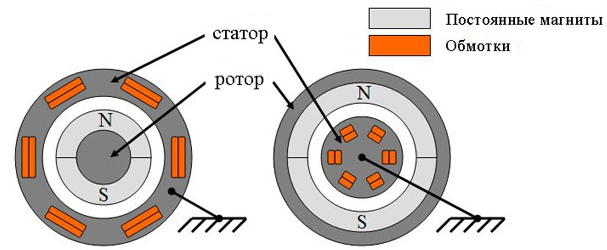
\includegraphics [scale=1] {intoutrot}
	\caption{Конструкции синхронного двигателя с постоянными магнитами: слева - стандартная, справа обращенная.}
	\label{fig:intoutrot}
\end{figure}

Ротор состоит из постоянных магнитов. В качестве постоянных магнитов используются материалы с высокой коэрцитивной силой.

\noindent По конструкции ротора синхронные двигатели делятся на:
\begin{enumerate}
\item электродвигатели с явно выраженными полюсами;
\item электродвигатели с неявно выраженными полюсами.
\end{enumerate}

Электродвигатель с неявно выраженными полюсами имеет равную индуктивность по продольной и поперечной осям $L_{d} = L_{q}$, тогда как у электродвигателя с явно выраженными полюсами поперечная индуктивность не равна продольной $L_{d} \neq L_{q}$.

\begin{figure}[ht]
	\centering
	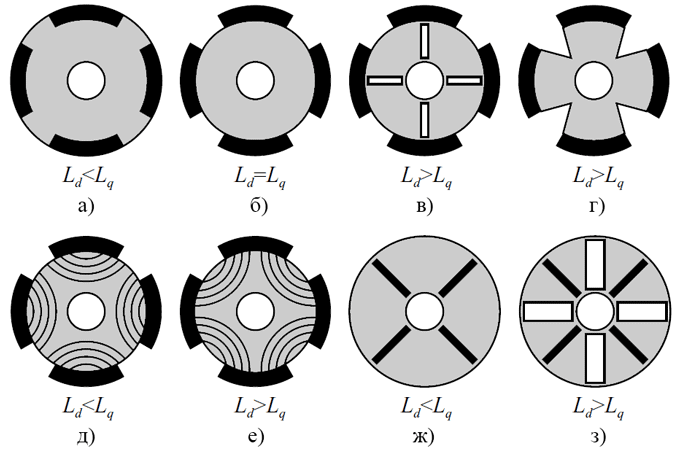
\includegraphics [scale=0.7] {rotor_saliency}
	\caption{Сечение роторов с разным отношением Ld/Lq. Черным обозначены магниты. На рисунке д, е представлены аксиально-расслоенные роторы, на рисунке в и з изображены роторы с барьерами.}
	\label{fig:rotor_saliency}
\end{figure}

Также по конструкции ротора СДПМ делятся на:
синхронный двигатель c поверхностной установкой постоянных магнитов
(англ. SPMSM - surface permanent magnet synchronous motor);
синхронный двигатель со встроенными (инкорпорированными) магнитами
(англ. IPMSM - interior permanent magnet synchronous motor).


\begin{figure}[ht]
	{\centering
		\hfill
		\subbottom[List-of-Figures entry][\label{fig:rotor_spmsm}]{%
			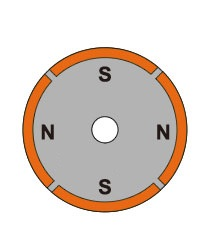
\includegraphics[width=0.35\linewidth]{rotor_spmsm}}
		\hfill
		\subbottom[\label{fig:rotor_ipmsm}]{%
			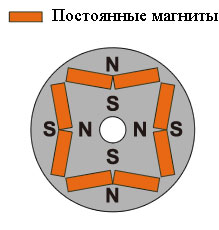
\includegraphics[width=0.35\linewidth]{rotor_ipmsm}}
		\hfill
	}
	\legend{а) Ротор синхронного двигателя c поверхностной установкой постоянных магнитов; б) Ротор синхронного двигателя со встроенными магнитами.}
	\caption{Конструкции ротора СДПМ}
	\label{fig:rotor_pmsm}
\end{figure}

Статор состоит из корпуса и сердечника с обмоткой. Наиболее распространены конструкции с двух- и трехфазной обмоткой.

\noindent В зависимости от конструкции статора синхронный двигатель с постоянными магнитами бывает:
\begin{itemize}
\item с распределенной обмоткой;
\item с сосредоточенной обмоткой.
\end{itemize}

Распределенной называют такую обмотку, у которой число пазов на полюс и фазу $Q = 2, 3,...., k$.
Сосредоточенной называют такую обмотку, у которой число пазов на полюс и фазу $Q = 1$. При этом пазы расположены равномерно по окружности статора. Две катушки, образующие обмотку, можно соединить как последовательно, так и параллельно. Основной недостаток таких обмоток - невозможность влияния на форму кривой ЭДС.
Представленное исследование рассматривает в качестве объекта синхронные двигатели с постоянными магнитами с поверхностной установкой постоянных магнитов (англ. SPMSM) и концентрированной обмоткой, так как данный тип моторов является наиболее подходящим для электротранспорта по следующим критериям: 

\begin{itemize}
\item высокий КПД
\item высокие показатели момента на низких скоростях
\item простота управления
\end{itemize}

В отличии от СДПМ с распределенной обмоткой, электромотор с концентрированной имеет более низкий вес (так как распределенная обмотка укладывается "в нахлест"), что особенно важно, так как конечный вес электромобиля напрямую влияет на запас хода на одном заряде и, как следствие, на эффективность работы всей системы в целом


\section{Постановка задач диссертационной работы}
\label{sec:ch1/sec3}


Сошлёмся на библиографию.
Одна ссылка: \cite[с.~54]{Sokolov}\cite[с.~36]{Gaidaenko}.
Две ссылки: \cite{Sokolov,Gaidaenko}.
Много ссылок: %\cite[с.~54]{Lermontov,Management,Borozda} % такой «фокус»
%вызывает biblatex warning относительно опции sortcites, потому что неясно, к
%какому источнику относится уточнение о страницах, а bibtex об этой проблеме
%даже не предупреждает
\cite{Lermontov, Management, Borozda, Marketing, Constitution, FamilyCode,
Gost.7.0.53, Razumovski, Lagkueva, Pokrovski, Methodology, Nasirova, Berestova,
Kriger}%
\ifnumequal{\value{bibliosel}}{0}{% Примеры для bibtex8
    \cite{Sirotko, Lukina, Encyclopedia}%
}{% Примеры для biblatex через движок biber
    \cite{Sirotko2, Lukina2, Encyclopedia2}%
}%
.
И~ещё немного ссылок:
\cite{Article,Book,Booklet,Conference,Inbook,Incollection,Manual,Mastersthesis,
Misc,Phdthesis,Proceedings,Techreport,Unpublished}
% Следует обратить внимание, что пробел после запятой внутри \cite{}
% обрабатывается ожидаемо, а пробел перед запятой, может вызывать проблемы при
% обработке ссылок.
\cite{medvedev2006jelektronnye, CEAT:CEAT581, doi:10.1080/01932691.2010.513279,
Gosele1999161,Li2007StressAnalysis, Shoji199895, test:eisner-sample,
test:eisner-sample-shorted, AB_patent_Pomerantz_1968, iofis_patent1960}
\ifnumequal{\value{bibliosel}}{0}{% Примеры для bibtex8
}{% Примеры для biblatex через движок biber
    \cite{patent2h, patent3h, patent2}%
}%
.

\ifnumequal{\value{bibliosel}}{0}{% Примеры для bibtex8
Попытка реализовать несколько ссылок на конкретные страницы
для \texttt{bibtex} реализации библиографии:
[\citenum{Sokolov}, с.~54; \citenum{Gaidaenko}, с.~36].
}{% Примеры для biblatex через движок biber
Несколько источников (мультицитата):
% Тут специально написано по-разному тире, для демонстрации, что
% применение специальных тире в настоящий момент в biblatex приводит к непоказу
% "с.".
\cites[vii--x, 5, 7]{Sokolov}[v"--~x, 25, 526]{Gaidaenko}[vii--x, 5, 7]{Techreport},
работает только в \texttt{biblatex} реализации библиографии.
}%

Ссылки на собственные работы:~\cite{vakbib1, confbib1}

Сошлёмся на приложения: Приложение \ref{app:A}, Приложение \ref{app:B2}.

Сошлёмся на формулу: формула \eqref{eq:equation1}.

Сошлёмся на изображение: рисунок \ref{fig:knuth}.

Стандартной практикой является добавление к ссылкам префикса, характеризующего тип элемента.
Это не является строгим требованием, но позволяет лучше ориентироваться в документах большого размера.
Например, для ссылок на рисунки используется префикс \textit{fig},
для ссылки на таблицу -- \textit{tab}.

В таблице \ref{tab:tab_pref} приложения \ref{app:B4} приведён список рекомендуемых
к использованию стандартных префиксов.

\section{Формулы} \label{sec:ch1/sec0}

Благодаря пакету \textit{icomma}, \LaTeX~одинаково хорошо воспринимает
в~качестве десятичного разделителя и запятую ($3,1415$), и точку ($3.1415$).

\subsection{Ненумерованные одиночные формулы} \label{subsec:ch1/sec3/sub1}

Вот так может выглядеть формула, которую необходимо вставить в~строку
по~тексту: $x \approx \sin x$ при $x \to 0$.

А вот так выглядит ненумерованая отдельностоящая формула c подстрочными
и надстрочными индексами:
\[
(x_1+x_2)^2 = x_1^2 + 2 x_1 x_2 + x_2^2
\]

При использовании дробей формулы могут получаться очень высокие:
\[
  \frac{1}{\sqrt{2}+
  \displaystyle\frac{1}{\sqrt{2}+
  \displaystyle\frac{1}{\sqrt{2}+\cdots}}}
\]

В формулах можно использовать греческие буквы:
\[
\alpha\beta\gamma\delta\epsilon\varepsilon\zeta\eta\theta\vartheta\iota\kappa%
\lambda\\mu\nu\xi\pi\varpi\rho\varrho\sigma\varsigma\tau\upsilon\phi\varphi%
\chi\psi\omega\Gamma\Delta\Theta\Lambda\Xi\Pi\Sigma\Upsilon\Phi\Psi\Omega
\]

Для красивых дробей (например, в индексах) в
\verb+userstyles.tex+ диссертации добавлен макрос
\verb+\slantfrac+, благодаря которому можно
писать $\slantfrac{1}{2}$ вместо $1/2$.

\subsection{Ненумерованные многострочные формулы} \label{subsec:ch1/sec3/sub2}

Вот так можно написать две формулы, не нумеруя их, чтобы знаки <<равно>> были
строго друг под другом:
\begin{align}
  f_W & =  \min \left( 1, \max \left( 0, \frac{W_{soil} / W_{max}}{W_{crit}} \right)  \right), \nonumber \\
  f_T & =  \min \left( 1, \max \left( 0, \frac{T_s / T_{melt}}{T_{crit}} \right)  \right), \nonumber
\end{align}

Выровнять систему ещё и по переменной $ x $ можно, используя окружение
\verb|alignedat| из пакета \verb|amsmath|. Вот так:
\[
    |x| = \left\{
    \begin{alignedat}{2}
        &&x, \quad &\text{eсли } x\geqslant 0 \\
        &-&x, \quad & \text{eсли } x<0
    \end{alignedat}
    \right.
\]
Здесь первый амперсанд (в исходном \LaTeX\ описании формулы) означает
выравнивание по~левому краю, второй "--- по~$ x $, а~третий "--- по~слову
<<если>>. Команда \verb|\quad| делает большой горизонтальный пробел.

Ещё вариант:
\[
    |x|=
    \begin{cases}
    \phantom{-}x, \text{если } x \geqslant 0 \\
    -x, \text{если } x<0
    \end{cases}
\]

Кроме того, для  нумерованых формул \verb|alignedat| делает вертикальное
выравнивание номера формулы по центру формулы. Например, выравнивание
компонент вектора:
\begin{equation}
 \label{eq:2p3}
 \begin{alignedat}{2}
{\mathbf{N}}_{o1n}^{(j)} = \,{\sin} \phi\,n\!\left(n+1\right)
         {\sin}\theta\,
         \pi_n\!\left({\cos} \theta\right)
         \frac{
               z_n^{(j)}\!\left( \rho \right)
              }{\rho}\,
           &{\boldsymbol{\hat{\mathrm e}}}_{r}\,+   \\
+\,
{\sin} \phi\,
         \tau_n\!\left({\cos} \theta\right)
         \frac{
            \left[\rho z_n^{(j)}\!\left( \rho \right)\right]^{\prime}
              }{\rho}\,
            &{\boldsymbol{\hat{\mathrm e}}}_{\theta}\,+   \\
+\,
{\cos} \phi\,
         \pi_n\!\left({\cos} \theta\right)
         \frac{
            \left[\rho z_n^{(j)}\!\left( \rho \right)\right]^{\prime}
              }{\rho}\,
            &{\boldsymbol{\hat{\mathrm e}}}_{\phi}\:.
\end{alignedat}
\end{equation}

Ещё об отступах. Иногда для лучшей <<читаемости>> формул полезно
немного исправить стандартные интервалы \LaTeX\ с учётом логической
структуры самой формулы. Например в формуле~\ref{eq:2p3} добавлен
небольшой отступ \verb+\,+ между основными сомножителями, ниже
результат применения всех вариантов отступа:
\begin{align*}
\backslash! &\quad f(x) = x^2\! +3x\! +2 \\
  \mbox{по-умолчанию} &\quad f(x) = x^2+3x+2 \\
\backslash, &\quad f(x) = x^2\, +3x\, +2 \\
\backslash{:} &\quad f(x) = x^2\: +3x\: +2 \\
\backslash; &\quad f(x) = x^2\; +3x\; +2 \\
\backslash \mbox{space} &\quad f(x) = x^2\ +3x\ +2 \\
\backslash \mbox{quad} &\quad f(x) = x^2\quad +3x\quad +2 \\
\backslash \mbox{qquad} &\quad f(x) = x^2\qquad +3x\qquad +2
\end{align*}

Можно использовать разные математические алфавиты:
\begin{align}
\mathcal{ABCDEFGHIJKLMNOPQRSTUVWXYZ} \nonumber \\
\mathfrak{ABCDEFGHIJKLMNOPQRSTUVWXYZ} \nonumber \\
\mathbb{ABCDEFGHIJKLMNOPQRSTUVWXYZ} \nonumber
\end{align}

Посмотрим на систему уравнений на примере аттрактора Лоренца:

\[
\left\{
  \begin{array}{rl}
    \dot x = & \sigma (y-x) \\
    \dot y = & x (r - z) - y \\
    \dot z = & xy - bz
  \end{array}
\right.
\]

А для вёрстки матриц удобно использовать многоточия:
\[
\left(
  \begin{array}{ccc}
    a_{11} & \ldots & a_{1n} \\
    \vdots & \ddots & \vdots \\
    a_{n1} & \ldots & a_{nn} \\
  \end{array}
\right)
\]

\subsection{Нумерованные формулы} \label{subsec:ch1/sec3/sub3}

А вот так пишется нумерованая формула:
\begin{equation}
  \label{eq:equation1}
  e = \lim_{n \to \infty} \left( 1+\frac{1}{n} \right) ^n
\end{equation}

Нумерованых формул может быть несколько:
\begin{equation}
  \label{eq:equation2}
  \lim_{n \to \infty} \sum_{k=1}^n \frac{1}{k^2} = \frac{\pi^2}{6}
\end{equation}

Впоследствии на формулы (\ref{eq:equation1}) и (\ref{eq:equation2}) можно ссылаться.

Сделать так, чтобы номер формулы стоял напротив средней строки, можно,
используя окружение \verb|multlined| (пакет \verb|mathtools|) вместо
\verb|multline| внутри окружения \verb|equation|. Вот так:
\begin{equation} % \tag{S} % tag - вписывает свой текст
  \label{eq:equation3}
    \begin{multlined}
        1+ 2+3+4+5+6+7+\dots + \\
        + 50+51+52+53+54+55+56+57 + \dots + \\
        + 96+97+98+99+100=5050
    \end{multlined}
\end{equation}

Используя команду \verb|\labelcref| из пакета \verb|cleveref|, можно
красиво ссылаться сразу на несколько формул
(\labelcref{eq:equation1,eq:equation3,eq:equation2}), даже перепутав
порядок ссылок \verb|(\labelcref{eq:equation1,eq:equation3,eq:equation2})|.
